\chapter*{Instalan pip}

\begin{enumerate}
	\item pertama-tama kita harus membuka cmd klik windows dan R secara bersamaan
	\begin{figure} [h]
	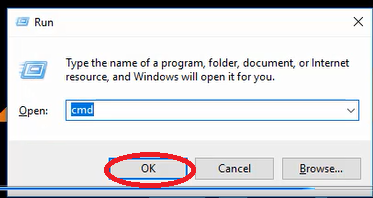
\includegraphics[width=5cm]{pip/0pip.png}
	\centering
	\end{figure}
	
	\item lalu ketikan cd download (tempat dimana kita menaruh hasil download-an pip)
	\begin{figure} [h]
	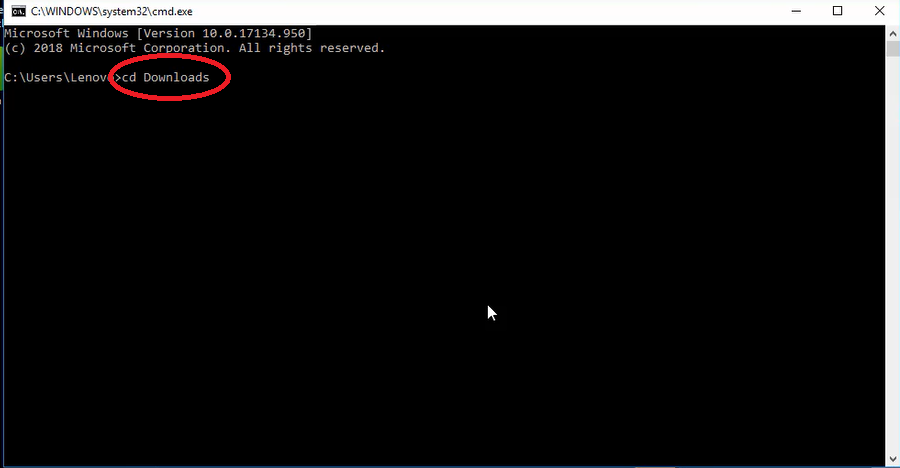
\includegraphics[width=5cm]{pip/1pip.png}
	\centering
	\end{figure}

	\item lalu ketikan python get-pip.py 
	\begin{figure} [h]
	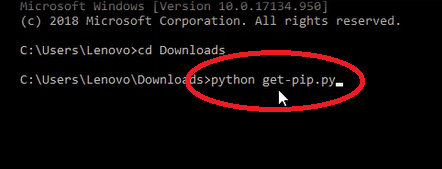
\includegraphics[width=5cm]{pip/2pip.png}
	\centering
	\end{figure}
	
	\item Tunggu sampai script keluar dan terdapat tulisan "succesfuly instaled"
	\begin{figure} [h]
	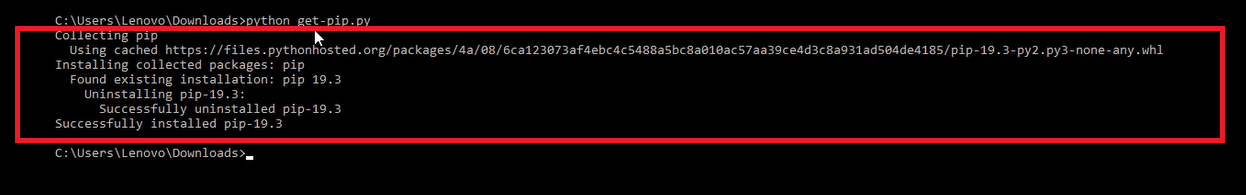
\includegraphics[width=6cm]{pip/3pip.png}
	\centering
	\end{figure}
	
	

\end{enumerate}
